\section{Cahier des charges}

\subsection{Définitions}

\begin{itemize}[label=\textbullet]
    \item \textbf{Micro-capsules}: petit cylindres en verre fermés des deux côtés (borosilicate). \\ 
    Diamètre extérieur = 2,8 ± 0,05 mm; \\
    Diamètre intérieur = 2,5 ± 0,05 mm; \\
    Longueur = 10 mm

    \item \textbf{Réacteurs}: Flacons en verre dimension: 11 mm, 12 x 32, 2 ml pour plaques « Para-Dox »\\
    REF: 11211-CASE  « Para-Dox »

    \item \textbf{Bloc de réaction}: Plaques « Para-Dox » avec 48 positions, Gen II, pour flacons 12 x 32
    
    \item \textbf{Glove-box}: Espace de travail sous atmosphère contrôlée, rempli d'azote à température 
    ambiante (environ 25 °C) et en surpression (+15 Pa par rapport à 1 Atm).
    \item \textbf{Cross contamination}: Contamination entre différents réactifs 
    causée par des restes dans le système d'ouverture ou par projection
\end{itemize}

\subsection{Analyse du besoin}

\begin{figure}[H]
    \centering
    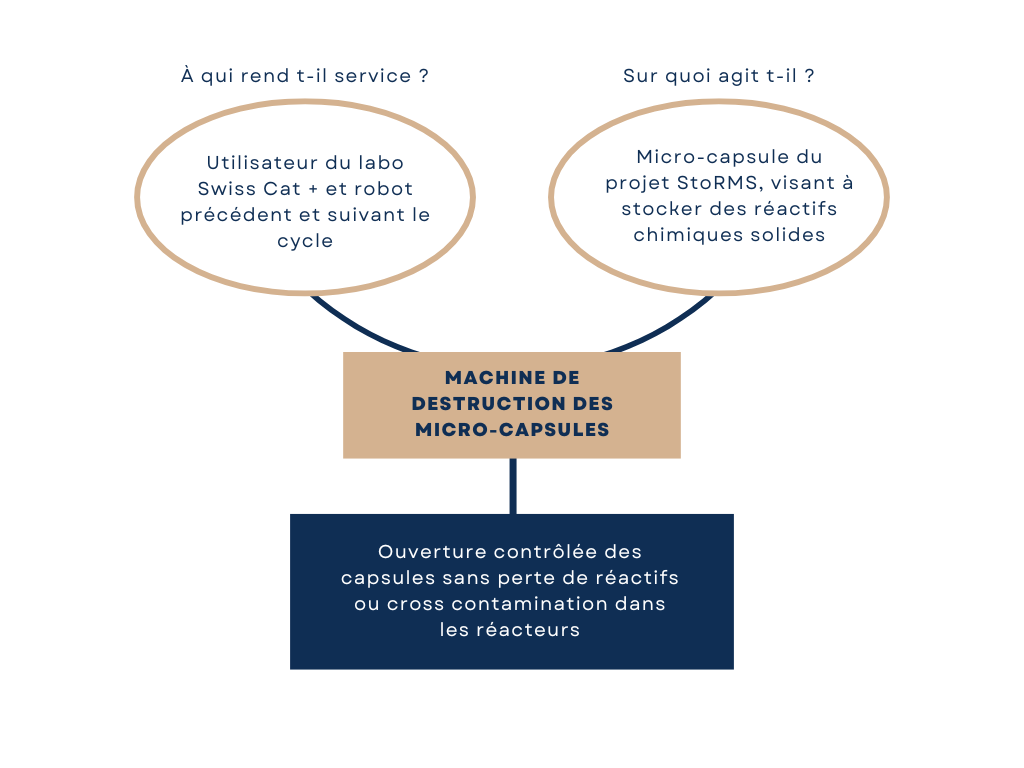
\includegraphics[width=15cm]{Images/Illustrations/CDH/Bete a corne.png}
    \label{fig:beteacorne}
    \caption{Diagramme bête à corne}
\end{figure}

\begin{table}[H]
    \centering
    \begin{tabular}{
    >{\columncolor[HTML]{FFFFFF}}l |
    >{\columncolor[HTML]{FFFFFF}}l }
    {\color[HTML]{000000} \textbf{\#}} & {\color[HTML]{000000} \textbf{Besoin}}         \\ \hline
    {\color[HTML]{000000} \textbf{1}} & {\color[HTML]{000000} Ouvrir des micro-capsules} \\ 
    \end{tabular}
    \caption{Liste des besoins du système}
    \label{tab:besoin}
    \end{table}

\subsection{Fonctions et exigences du système}
\subsubsection{Fonctions de services}

Les fonctions de services correspondes aux exigences principales du produits.

\begin{table}[H]
  \centering
  \begin{tabular}{cl|cl}
  \multicolumn{2}{l|}{\textbf{Fonctions de service}} &
    \multicolumn{2}{l}{\textbf{Exigences}} \\ \hline
  \multicolumn{1}{c|}{\textbf{FS 1}} &
    \begin{tabular}[c]{@{}l@{}}Doit être en mesure d'ouvrir plusieurs\\ micro-capsules dans un réacteur.\end{tabular} &
    \multicolumn{1}{c|}{\textbf{E 1}} &
    \begin{tabular}[c]{@{}l@{}}Ouverture des micro-capsules\\ contrôlée, sans contrainte sur \\ la présence de débris de verre.\end{tabular} \\ \hline
  \multicolumn{1}{c|}{\textbf{FS 2}} &
    \begin{tabular}[c]{@{}l@{}}Doit effectuer la fonction sur tout\\ les réacteurs de la plaque para-dox.\end{tabular} &
    \multicolumn{1}{c|}{\textbf{E 2}} &
    \begin{tabular}[c]{@{}l@{}}Répétabilité de la tâche\\ 48 fois par plaque.\end{tabular} \\ \hline
  \multicolumn{1}{c|}{\textbf{FS 3}} &
    \begin{tabular}[c]{@{}l@{}}Doit s’assurer de la libération\\ du réactif.\end{tabular} &
    \multicolumn{1}{c|}{\textbf{E 3}} &
    \begin{tabular}[c]{@{}l@{}}La masse de réactif libéré est \\ précise à 0.01 mg.\end{tabular}
  \end{tabular}
  \caption{Fonctions de service}
  \label{tab:fctsservice}
  \end{table}

\subsubsection{Fonctions techniques}

Les fonctions techniques corresponde aux caractéristiques techniques que doit intégrer le produit.

\begin{table}[H]
  \centering
  \begin{tabular}{cl|cl}
  \multicolumn{2}{l|}{\textbf{Fonctions techniques}} &
    \multicolumn{2}{l}{\textbf{Exigences}} \\ \hline
  \multicolumn{1}{c|}{\textbf{FT 1}} &
    \begin{tabular}[c]{@{}l@{}}Doit fonctionner dans \\ un environnement contrôlé.\end{tabular} &
    \multicolumn{1}{c|}{\textbf{E 5}} &
    \begin{tabular}[c]{@{}l@{}}Glove box rempli uniquement d'azote \\ à température ambiante (environ 25 °C)\\ et en surpression \\(+15 Pa par rapport à 1 Atm).\end{tabular} \\ \hline
  \multicolumn{1}{c|}{\textbf{FT 2}} &
    Doit être dépannable facilement. &
    \multicolumn{1}{c|}{\textbf{E 6}} &
    \begin{tabular}[c]{@{}l@{}}Accessibilité simple et adapté \\ à un laborantin de chimie.\end{tabular} \\ \hline
  \multicolumn{1}{c|}{\textbf{FT 3}} &
    \begin{tabular}[c]{@{}l@{}}Doit alerter l'utilisateur en cas de\\ défaillance et éviter l'endommagement\\ des appareils.\end{tabular} &
    \multicolumn{1}{c|}{\textbf{E 7}} &
    \begin{tabular}[c]{@{}l@{}}Capteurs ou système de sécurité \\ en cas de défaillance \\ ou conditions anormale.\end{tabular} \\ \hline
  \multicolumn{1}{c|}{\textbf{FT 4}} &
    \begin{tabular}[c]{@{}l@{}}Doit assurer la sécurité de l'utilisateur \\ en cas de défaillance.\end{tabular} &
    \multicolumn{1}{c|}{\textbf{E 8}} &
    Protection contre les débris de verre.
  \end{tabular}
  \caption{Fonctions techniques}
  \label{tab:fctstechnique}
  \end{table}

\subsubsection{Fonctions de contraintes}

Les fonctions de contraintes correspondent à des exigences imposé par le client ou par la configuration des lieux.

\begin{table}[H]
  \centering
  \begin{tabular}{cl|cl}
  \multicolumn{2}{l|}{\textbf{Fonctions de contrainte}} &
    \multicolumn{2}{l}{\textbf{Exigences}} \\ \hline
  \multicolumn{1}{c|}{\textbf{FC 1}} &
    \begin{tabular}[c]{@{}l@{}}Doit éviter la cross contamination\\ entre les réacteurs\end{tabular} &
    \multicolumn{1}{c|}{\textbf{E 9}} &
    Système anti-projection \\ \hline
  \multicolumn{1}{c|}{\textbf{FC 2}} &
    \begin{tabular}[c]{@{}l@{}} Doit fonctionner dans un espace \\ restreint.\end{tabular} &
  \multicolumn{1}{c|}{\textbf{E 10}} & 
    \begin{tabular}[c]{@{}l@{}}Dimensions maximal de travail: \\ 110 cm x 90 cm x 60 cm. \end{tabular}
  \end{tabular}
  \caption{Fonctions de contrainte}
  \label{tab:fctscontr}
  \end{table}




